\chapter[Projeto Eletrônico]{Projeto Eletrônico}

\section{Objetivo Específico}

Captar, condicionar e processar os dados obtidos através dos sensores internos e externos de um motor a combustão (FIAT 1.0 MPI), além de transmiti-los de forma precisa e sistematizada de acordo com requisitos não funcionais do SBTM (Software da Bancada de Testes de Motor)

\section{Requisitos}

O intuito de analisar eletronicamente os principais parâmetros de funcionamento de um motor implica na aplicação de um sistema de sensoriamento, tanto interno, quanto externo do motor. Com o passar dos anos e a evolução tecnológica este sensoriamento está cada vez mais completo. Os motores já saem de fábrica com uma grande oferta de sensores acoplados internamente \cite{techreport}. Estes sensores variam de acordo com modelo e fabricante do motor, mas normalmente apresentam as mesmas características para um mesmo parâmetro.

Os principais parâmetros de um motor a serem avaliados são:

\begin{itemize}
	\item Temperatura do óleo do motor;
	\item Temperatura do ar no coletor de admissão;
	\item Pressão do ar no coletor de admissão;
	\item Velocidade angular do eixo das árvores de manivelas;
	\item Posição angular da válvula borboleta;
	\item Fluxo de ar posterior a válvula borboleta;
	\item Quantidade de oxigênio presentes nos gases de exaustão.
\end{itemize}

Todos sensores que monitoram estes parâmetros já são acoplados ao motor no momento da fabricação, porém outros parâmetros importantes para análise devem ser considerados, são eles:

\begin{itemize}
	\item Temperatura de entrada da água no radiador;
	\item Temperatura de saída da água no radiador;
	\item Temperatura dos gases de combustão;
\end{itemize}

Estes parâmetros já não possuem um sensor monitorando-os, o que faz necessária sua implementação.

A relação da temperatura da água na entrada e saída do radiador apresenta a funcionalidade do radiador, ou seja, se realmente há transferência de calor entre motor e radiador.

Todos estes sensores são passivos e emitem os dados em forma de sinais elétricos, sendo eles, alguma relação de tensão e corrente de acordo com o parâmetro a ser monitorado. Como um dos requisitos deste projeto apresenta uma interação com um software, todos estes dados devem ser processados digitalmente, o que implica na utilização de um microcontrolador para a aquisição e processamento destes sinais e transmissão dos mesmos, de modo que o software possa interpretá-lo de forma fiel e precisa. 

O sinal que varia mais rapidamente em relação ao tempo é a velocidade angular das árvores de manivelas ou simplesmente o RPM (rotação por minuto) do motor, pois os sinais de temperatura e posição angular da válvula borboleta não variam tão rapidamente. O motor a ser analisado apresenta rotação máxima entre 6000 e 7000 rpm, transcrevendo isto para o domínio da frequência significa que a frequência máxima lida pelo sensor é de aproximadamente: 7000 rotações a cada 60 segundos.

\begin{equation}
	f = \frac{7000}{60} \cong 117 Hz	
\end{equation}

Com isso adotando-se o critério de \textit{Nyquist-Shanon} \cite{diniz2014processamento} a taxa mínima de amostragem deste sinal sem perda de informação é dada pelo dobro da frequência máxima do sinal amostrado, evitando o efeito de \textit{Aliasing} \cite{diniz2014processamento}. Portanto para estabelecer este critério o \textit{clock} mínimo do microcontrolador deve ser de 234 Hz.

Além disso tendo em vista que são ao total 10 sensores o microcontrolador deve ter ao menos 10 pinos GPIO (\textit {General Pruporse Inputs/Outpus}) para que o mesmo tenha acesso ao barramento com os dados do sensor. 

Por via de segurança é cabível que o usuário não esteja próximo ao motor no momento em que o mesmo esteja funcionando, portanto, uma aplicação via software para realizar a partida do motor, além do controle de velocidade, também abrange este projeto.

\section{Implementação}

Tendo em vista a quantidade de sensores a serem analisados e o estado crítico do controle do sistema de partida e aceleração do motor, cada um destes sistemas (aquisição de dados, controle) terá um microcontrolador dedicado que serão estruturados e organizados a partir de um servidor.

\subsection{Sistema de Aquisição}

Todo sistema de aquisição a ser implementado pode ser dividido em 4 módulos, apresentados na figura \ref{diagramaDeAquisicaoDeDados}

\begin{figure}[h!]
	\centering
	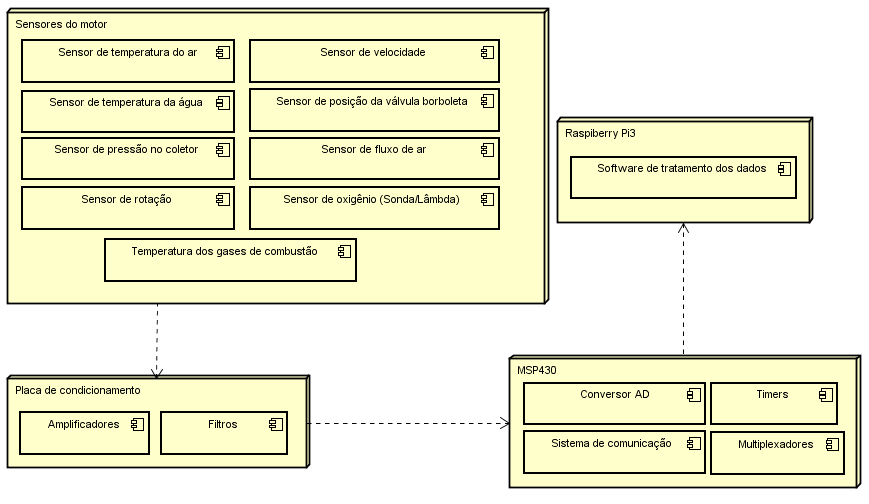
\includegraphics[keepaspectratio=true,scale= 0.7]{figuras/Diagrama.PNG}
	\caption{Diagrama de aquisição de dados}
	\label{diagramaDeAquisicaoDeDados}
\end{figure}

\subsection{Sensores}

Os sensores utilizados internamente no motor apresentam características específicas apresentadas na tabela x.
